\textit{Tabletop Game Prototype Language} é una nuova possibile sintassi 
per un linguaggio specializzato nella prototipizzazione dei giochi da tavolo,
proposto in questa tesi e illustrato nelle pagine successive.

\section{Nozioni Fondamentali}

\subsection{Identificatori}
Gli Identificatori sono una qualsiasi stringa di caratteri che inizia per un trattino basso "\_" o 
per lettera, opzionalmente seguiti da un qualsiasi ammontare di lettere o numeri senza spazi. \\
Un identificatore per essere legale deve essere unico all'interno del suo ambito di visibilità,
questo significa che deve essere diverso sia dagli altri identificatori ma anche da operatori e clausole.  

\subsection{Operatori e Clausole}
Gli operatori e le clausole sono delle parole chiave o simboli riservati che permettono rispettivamente
la costruzione delle espressioni e delle istruzioni.

\subsection{Blocchi}
I blocchi sono un insieme struttura d'istruzioni, tag e altri blocchi.
Un blocco si definisce come tutto il contenuto all'interno di una coppia di parentesi graffe,
rispettivamente aperta e chiusa. 
\\
Il blocco delimita l'ambito, o scope, e vita di una variabile definita al suo interno ovvero
il suo campo d'azione, che parte dalla riga dov'è stata dichiarata fino alla fine del blocco 
che contiene la sua dichiarazione.
\\
La Visibilità di una variabile si estende a tutti gli ambiti figli del blocco di dichiarazione, 
dove figlio significa definito all'interno del padre (annidato).
 
\subsection{Tags}
I Tag sono delle parole chiave riservate che modificano il comportamento del blocco associato, 
ogni tag descrive cosa è permesso definire al suo interno. \\
All'interno della proposta è possibile che si trovi la dicitura blocco tag come abbreviazione
per indicare la coppia tag e relativo blocco associato.
 
\subsection{Commenti}
I commenti sono linee di codice che vengono ignorate durante l'esecuzione del programma. \\
Per commentare una riga è sufficiente inserire una doppia barra "//", qualsiasi scritta oltre 
le due barre è considerata parte del commento.

\section{Primitive del linguaggio}
Tabletop Game Prototype Language si basa su un insieme di primitive da cui sono costruire tutte 
le funzionalità del linguaggio.
 
\subsection{Oggetti}
Un oggetto è un'istanza di una certa classe, un blocco di memoria che viene allocato e configurato secondo
le specifiche definite dalla classe. \\
Gli oggetti hanno due comportamenti principali, ispirati dal linguaggio C\# \cite{CSharpLang}:
\paragraph{Oggetti valore} Detti anche Value objects, 
si riferiscono direttamente al valore. Quando avviene una copia dell'oggetto
viene creata una nuova istanza della stessa tipologia di oggetto che contiene lo stesso valore.
Il comportamento degli oggetti valore è utilizzato principalmente per i tipi primitivi come number, string, bool. 
\paragraph{Oggetti riferimento} Detti anche Reference objects, 
si riferiscono al blocco di memoria che gli è stato allocato, segue che, 
quando un reference object è copiato in una nuova variabile, nel nuovo oggetto si copierà 
il riferimento alla zona di memoria a cui l'oggetto originale si riferisce, evitando di allocare una
nuova zona di memoria. 
\\
Una conseguenza importante del meccanismo dei riferimenti è che qualsiasi cambiamento effettuato su un
oggetto riferimento sarà rispecchiato da tutti gli altri reference objects che possiedono lo stesso riferimento
al blocco di memoria

\subsection{Tipi primitivi}
I tipi primitivi sono degli oggetti valore particolari che rappresentano i valori puri del linguaggio come
i numeri, le stringhe di testo, i valori booleani.

\subsubsection{Numeri}
I numeri sono rappresentati dal tipo primitivo "number" che accoglie un qualsiasi numero tale che
sia compreso tra \( \pm5.0*10^{-324} \) e \(\mp 1.7*10^{308}\) con una precisione tra le 15 e le 17
cifra, il tipo number equivale al tipo double presente in linguaggi come C, C\#, ecc...

\subsubsection{Stringa}
Il tipo stringa, o string, rappresenta una qualsiasi successione di caratteri codificata in UTF-16, 
non ha una lunghezza massima predefinita.
I valori string sono immutabili (ovvero non è modificabile), quando si eseguono delle espressioni
che andrebbero a modificare il valore di una stringa, viene instanziata una nuova stringa con il valore
modificato.

\subsubsection{Booleano}
Il tipo booleano, o bool, rappresenta una decisione binaria vera o falsa.
Le variabili di tipo booleano dunque possono assumere due singoli valori rispettivamente 
rappresentati dalle parole chiave "true" per il valore vero e "false" per il valore falso.

\subsubsection{Null}
Il valore null non è un tipo primitivo in sé ma serve per indicare l'assenza del valore in una variabile,
Ogni tipo può assumere il valore null.

\subsection{Collezioni} % Aggiungere la sintassi generica, ispirata dalla sintassi dei generics di c# e java
Una collezione é un qualsiasi gruppo di oggetti che sono rappresentati come una singola unità,
in altri linguaggi esistono varie tipologie di collezioni come array, hashtables, vectors, ect\dots \\
Attualmente sono supportate tre tipologie: lista, table, stack, la cui sintassi è inspirata dalle
collezioni generiche del linguaggio C\#

\subsubsection{Liste}
Le liste forniscono un insieme di oggetti accessibili tramite indici numerici interi, che mantiene l'ordine d'inserimento. \cite{CSharpLang} \\
Non hanno una dimensione fissa ma si adattano in base al numero di oggetti che contengono. \\
Per dichiarare una lista si utilizza il tipo lista, composto dalla parola chiave 
\lstinline|List| e una coppia di parentesi angolate con all'loro interno Il tipo degli 
oggetti che si vuole raggruppare \lstinline|List<<tipo>>|. \\
L'inizializzazione é effettuata tramite un blocco in cui è definibile un elenco di 
espressioni, dello stesso tipo definito nella dichiarazione, separate da una virgola.
\begin{lstlisting}
List<<tipo>> <identificatore> = {
    <espressione tipo>,
    <espressione tipo>,
    ...
};
\end{lstlisting}
La lista accetta anche valori nulli, l'indice corrispondente presenterà un valore nullo quando si farà accesso. 
Le seguenti funzionalità sono supportate dalle liste: 
\begin{center}
\begin{tabularx}{\linewidth}{| X | c | X |}
    \hline 
    Lunghezza & \lstinline|<lista>.lenght| & calcola il numero d'indici occupati \\
    \hline
    Accesso & \lstinline|<lista>[<numero>]| & accede all'indice numero, se non é intero la parte decimale verrà
     troncata. \\
    \hline
    Aggiungere \newline una lista & \lstinline|<lista>.append(<lista>)| & aggiunge tutti gli elementi di una lista in code \\
    \hline
    Rimuovere tutto & \lstinline|<lista>.clear()|& rimuove tutti gli oggetti dalla lista\\
    \hline
    Contiene valore & \lstinline|<lista>.contains(<oggetto>)| & ritorna true se la lista contiene lo stesso 
    oggetto, falso altrimento \\ 
    \hline
    Trova indice & \lstinline|<lista>.indexOf(<oggetto>)|& restituisce l'indice del primo oggetto corrispondente,
    altrimenti -1 \\
    \hline
    Rimuovi elemento & \lstinline|<lista>.remove(<oggetto>)|& rimuove il primo oggetto corrispondente che trova,
    sposta il resto della lista avanti di una posizione \\
    \hline    
    Rimuovi elemento all'indice & \lstinline|<lista>.removeAt(<indice>)|& rimuove l'oggetto all'indice corrispondente,
    sposta il resto della lista avanti di una posizione \\
    \hline    
    Ordinamento \newline casuale & \lstinline|<lista>.shuffle()| & mescola casualmente la lista \\
    \hline
    Copia & \lstinline|<lista>.copy()| & crea una copia shallow della lista \\
    \hline
\end{tabularx}
\end{center}

\newpage
\subsubsection{Table}
Ispirata dalla omonima struttura dati del famoso linguaggio di scripting LUA \cite{LUA},
sono array associativi, ovvero che possono essere indicizzati non solo con dei 
numeri ma con qualsiasi oggetto eccetto il valore null. \\
Per dichiarare una table si utilizza il tipo table, composto dalla parola chiave
\lstinline|Table| e una coppia di parentesi angolate con all'loro interno il tipo degli 
oggeti che si vuole raggruppare \lstinline|Table<<tipo>>|. \\
L'inizializzazione é effettuata tramite un blocco in cui sono definibili delle coppie
di espressioni separate da una virgola.
\begin{lstlisting}
Table<<tipo>> <identificatore> = {
    {<espressione chiave>, <espressione valore>},
    {<espressione chiave>, <espressione valore>},
    ...
};
\end{lstlisting}
Le espressioni saranno valutate nel momento in cui la variabile sarà inizializzata,
per avere una definizione legale della table le espressioni valore devono avere 
lo stesso tipo definito nella dichiarazione. \\
In caso una espressione chiave venga valutata an null, il programma terminerà con errore.
Le seguenti funzionionalità sono supportate per le table: \\
\begin{center}
\begin{tabularx}{\linewidth}{| X | c | X |}
    \hline 
    Funzione & Sintassi & Descrizione \\
    \hline 
    Lunghezza & \lstinline|<table>.length| & calcola quante coppie sono presenti all'interno \\
    \hline
    Accesso & \lstinline|<table>[<chiave>]| & ritorna il valore o null se la chiave non é presente \\ 
    \hline
    Rimuovere tutto & \lstinline|<table>.clear()| & elimina tutte le coppie contenute nella table \\
    \hline
    Copia & \lstinline|<table>.copy()| & crea una copia shallow della table \\
    \hline
    Rimozione coppia & \lstinline|<table>[<chiave>]| = null & rimuove una coppia chiave/valore dalla table \\
    \hline
\end{tabularx}
\end{center}

\newpage
\subsubsection{Stack}
Gli stack sono una raccolta di oggetti di tipo LIFO (Last-in, First-out) \cite{CSharpLang}.
Per dichiarare uno stack si utilizza il tipo stack, composto dalla parola chiave \lstinline|Stack|
e una coppia di parentesi angolate con all'loro interno il tipo degli oggetti che si vuole raggruppare
\lstinline|Stack<<tipo>>|. \\
L'inizializzazione é effettuata tramite un blocco in cui è definibile un elenco di espressioni,
dello stesso tipo definito nella dichiarazione, separate da una virgola.
\begin{lstlisting}
Stack<<tipo>> <identificatore> = {
    <espressione tipo>,
    <espressione tipo>,
    ...
};
\end{lstlisting}
Lo stack accetta valori nulli nelle funzioni di push ma non lo aggiunge allo stack, trattandolo quindi
come un noop (no operation). \\ 
Le seguenti funzionalità sono supportate: 
\begin{center}
\begin{tabularx}{\linewidth}{|X|c|X|}
    \hline
    Lunghezza & \lstinline|<stack>.lenght()|& Restituisce il numero di oggetti nello stack \\
    \hline
    Inserimento & \lstinline|<stack>.push(<tipo>)| & Inserisce in cima allo stack un oggetto \\
    \hline
    Inserimento in fronte& \lstinline|<stack>.push_front(<tipo>)| & Inserisce in fronte allo stack un oggetto \\
    \hline
    Pop & \lstinline|<stack>.pop()| & Rimuovare e restituisce l'oggetto in cima allo stack\\
    \hline
    Pop in fronte& \lstinline|<stack>.pop_front()| & Rimuove e resistuisce l'oggeto in fronte allo stack\\
    \hline
    Copia & \lstinline|<stack>.clone()| & Restituisce una copia shallow dello stack \\
    \hline
    Ordinamento casuale & \lstinline|<stack>.shuffle()| & Mescola casualmente lo stack\\
    \hline
\end{tabularx}
\end{center}

\newpage
\subsection{Espressioni}
Una espressione è una qualsiasi operazione che coinvolge zero o più operatori e uno o più operandi 
(o espressioni) che può essere valutata all’interno del linguaggio. \\
Ogni espressione ha un tipo di ritorno che indica il tipo dell’oggetto che sarà restituito dopo la valutazione 
dell’espressione. \\
Gli operatori sono predefiniti e si possono trovare tutti nella lista di definizione degli operatori. \\
Le espressioni vengono classificate in base al tipo di ritorno o al numero di operatori. \\
Nella definizione delle espressioni, con il tipo del valore si intende una qualsiasi espressione che ritorna 
un oggetto dello stesso tipo.

\subsubsection{Espressioni letterali}
Le espressioni letterali sono un qualsiasi valore puro di un tipo primitivo (number, string, bool). \\ 
Seguono alcuni esempi di espressioni letterali separata dalla virgola: 1, 0.2, “hello world”, true, false

\subsubsection{Espressioni matematiche}
Le espressioni matematiche sono una qualsiasi operazione che coinvolga degli operatori matematici,
hanno come tipo di ritorno il tipo number.
\\
Le seguenti sono tutte espressioni matematiche:
\begin{itemize}
    \item Addizione \lstinline|<numero> + <numero>|
    \item Sottrazione \lstinline|<numero> - <numero>|
    \item Prodotto \lstinline|<numero> * <numero>|
    \item Divisione \lstinline|<numero> / <numero>|
    \item Potenza \lstinline|<numero> ^ <numero>|
    \item Modulo \lstinline|<numero> % <numero>|
\end{itemize}
l'ordine di precedenza per la valutazione segue quello matematico:
\begin{enumerate}
    \item Potenza
    \item Prodotto, divisione e Modulo
    \item Addizione e Sottrazione
\end{enumerate}

\subsubsection{Espressioni di confronto}
Le espressioni di confronto coinvolgono gli operatori di maggioranza e minoranza, stretta e larga,
il tipo di ritorno dell'espressione è un booleano il cui valore è il risultato del confronto:
\begin{itemize}
    \item Minore di \lstinline|<espressione> < <espressione>|
    \item Maggiore di \lstinline|<espressione> > <espressione>|
    \item Minore uguale di \lstinline|<espressione> <= <espressione>|
    \item Maggiore uguale di \lstinline|<espressione> >= <espressione>|
\end{itemize}
\textbf{Il tipo di ritorno dei due operandi deve essere il medesimo}

\subsubsection{Espressioni di uguaglianza}
Le espressioni di uguaglianza coinvolgono gli operatori di uguaglianza, 
il tipo di ritorno dell'espressione è booleano il cui valore è il risultato dell'uguaglianza:
\begin{itemize}
    \item Uguale a \lstinline|<espressione> == <espressione>|
    \item Diverso da \lstinline|<espressione> != <espressione>|
\end{itemize}
Come per le espressioni di confronto, il tipo dei due operandi deve essere il medesimo
per avere una espressione di uguaglianza legale.

\subsubsection{Espressioni logiche condizionali}
Le espressioni logiche condizionali coinvolgono gli operatori logici AND e OR,
il tipo di ritorno dell'espressione è booleano il cui valore è il risultato dell'operazione logica:
\begin{enumerate}
    \item AND \lstinline|<booleano> && <booleano>|
    \item OR \lstinline=<booleano> || <booleano>=
\end{enumerate}
Le espressioni logiche condizionali cercano di valutare il minimo possibile per ottimizzare i controlli.
Se una espressione si rivela vera o falsa alla valutazione del primo operando, l'operazione non 
valuterà il secondo operando ma ritornerà direttamente il corrispettivo risultato.

\subsubsection{Espressioni logiche binarie}
Le espressioni logiche binarie sono simili alle espressioni logiche condizionali ma valutano sempre
entrambi gli operandi
\begin{enumerate}
    \item AND \lstinline|<booleano> & <booleano>|
    \item OR \lstinline=<booleano> | <booleano>=
    \item XOR \lstinline|<booleano> ^ <booleano>|
    \item NOT \lstinline|!<booleano>|
\end{enumerate}

\subsubsection{Espressioni di accesso}
Le espressioni di accesso permettono d'interagire con i valori contenuti all'interno delle variabili.
In base all'espressione si accederà a tipologie di oggetti diversi.

\begin{itemize}
    \item 
    {
        Accesso a membro: \lstinline|<oggetto>.<membro>| \\ 
        utilizza operatore di accesso \lstinline|.| per accedere
        al valore di uno specifico membro di un oggetto.
        Il tipo di ritorno dell'espressione è il tipo del membro a cui si sta accedendo.
    }
    \item 
    {
        Accesso tramite indice: \lstinline|<collezione>[<chiave>]| \\ 
        utilizza l'operatore di accesso tramite un indice
        \lstinline|[<chiave>]| per accedere alla variabile associata della lista. \\
        Ha come tipo di ritorno lo stesso tipo degli oggetti della lista.
    }
    \item 
    {
        Accesso a variabile: \lstinline|<identificatore>| \\ 
        l'identificatore unico deve appartenere ad variabile
        per poter essere legale. Accede al valore contenuto nella variabile, il tipo di ritorno dell'espressione
        è lo stesso tipo della variabile a cui si sta accedendo
    }
\end{itemize}

\subsubsection{Espressione tipo} 
Ispirate dal linguaggio C\# per la loro chiarezza,
le espressioni tipo o type expression sono tutte quelle espressioni che si occupano della 
gestione dei tipi degli oggetti:
\begin{itemize}
    \item
    {
        Controllo del tipo: \lstinline|<oggetto> is <tipo>| \\
        controlla se l'oggetto è del tipo richiesto.
        L'espressione ha come tipo di ritorno un valore booleano cui valore corrisponde il risultato del controllo:
        vero se l'oggetto è del tipo richiesto, falso altrimenti.
    }
    \item 
    {
        Conversione del tipo, type casting: \lstinline|<oggetto> as <tipo>| \\
        il type casting é utilizzato
        per convertire un oggetto in un oggetto di tipo diverso, il tipo di ritorno é lo stesso del tipo richiesto.
        Nel caso la conversione sia ammissibile l'espressione ristornerà il nuovo oggetto con il tipo prestabilito,
        in caso contrario sarà ritornato un valore nullo.
    }
\end{itemize}

\subsubsection{Espressioni d'istanziazione}
L'espressione d'istanziazione \lstinline|new <tipo>()| è usata per creare una nuova istanza del tipo
richiesto, il tipo di ritorno corrisponde al tipo richiesto.
\\
L'istanziazione di un oggetto può essere seguita da una lista d'inizializzazione per popolare 
velocemente con dei valori il nuovo oggetto.

\subsubsection{Espressione d'assegnamento}
\lstinline|<espressione di accesso> = <espressione>| \\
L'espressione di assegnamento è utilizzata per assegnare il risultato di un espressione
a una variabile, attributo o a uno specifico indice di una lista. \\
Per avere un espressione di assegnamento legale è necessario che i tipi di ritorno
delle due espressioni siano gli stessi. \\
Il tipo di ritorno dell'espressione è nullo.

\subsubsection{Espressione di chiamata}
\lstinline|<identificatore>(<lista argomenti>)| \\
L'espressione di chiamata è utilizzata per chiamare l'esecuzione di della funzione con lo 
stesso identificatore con degli specifici argomenti definiti nella lista degli argomenti. \\
Il tipo di ritorno dell'espressione corrisponde al tipo di ritorno della funzione. \\
L'espressione di chiamata è approfondita in \ref*{ChiamataFunzione}

\subsubsection{Espressione giocatore} \label{EspressioniGiocatore}
Una espressione giocatore, o player expression, è un'espressione speciale utilizzata per ritornare 
un oggetto giocatore.  \\
Gli oggetti giocatori sono identificati tramite un numero partendo da zero fino al numero di giocatori meno uno,
questi identificatori numerici possono essere utilizzati all'interno delle espressioni giocatore, che equivale 
a una espressione matematica il cui risultato è ristretto per poter essere mappato a un giocatore. \\
La funzione che si occupa di riportare il risultato dell'espressione matematica nell'intervallo di 
mappatura dei giocatori è la seguente
\[
\begin{cases}
    r \% P  & r >= 0 \\
    (P - |r| \% P) \% P & r < 0
\end{cases}
\] 
Dove:
\begin{itemize}
    \item r: è il risultato dell'equivalente espressione matematica
    \item P: è il numero di giocatori
    \item \%: è l'operatore modulo
\end{itemize}

\subsubsection{Ordine di precedenza}
L'ordine standard (senza modificatori di precedenza) di valutazione delle espressioni è il seguente:
\begin{enumerate}
    \item Espressioni d'istanziazione
    \item Espressioni di chiamata
    \item Espressioni di accesso
    \item Espressioni matematiche
    \item Espressioni giocatore
    \item Espressioni di confronto
    \item Espressioni di uguaglianza 
    \item Espressioni logiche binarie 
    \item Espressioni logiche condizionali 
    \item Espressioni di assegnamento
\end{enumerate}
Se non specificato altrimenti le espressioni all'interno di una stessa categoria 
si risolvo da sinistra verso destra. \\
Qualsiasi espressione può essere inserita all'interno di parentesi tonde per aumentare 
la priorità di valutazione, la valutazione partirà delle espressioni maggiormente innestate.

\newpage
\subsection{Istruzioni}
Le istruzioni, o statements, sono i macro comandi del linguaggio, ovvero una combinazione 
di clausole ed espressioni usate per adempire a un compito preciso.
Le istruzioni devono terminare con il carattere \lstinline|;|, ma nel caso sia possibile definire
un blocco d'istruzioni associato è possibile omettere il \lstinline|;|

\subsubsection{Istruzione di ritorno}
\lstinline|return [<espressione>];| \\
L’istruzione di ritorno è utilizzata per finire l’esecuzione di un effetto,
ritornando il controllo al codice che ha chiamato la funzione,
restituendo (o no) un risultato in base al tipo di ritorno della funzione. \\
Il risultato restituito proviene dalla valutazione della espressione definita nella istruzione,
nel caso si abbia un tipo di ritorno senza tipo bisogna omettere la espressione.

\subsubsection{Istruzione espressione}
\lstinline|<espressione>;| \\
l'istruzione espressione, o expression statement, serve per eseguire una certa espressione; 


\subsubsection{Istruzione di dichiarazione}
\lstinline|<tipo> <identificatore> = <espressione>;| \\
L'istruzione di dichiarazione è utilizzata per definire delle nuove variabili del tipo 
richiesto e inizializzate con il risultato dell'espressione alla destra dell'operatore d'assegnamento. \\
Le variabili dichiarate sono utilizzabili dopo la loro dichiarazione tramite l'identificatore, ovvero
tramite una espressione di accesso. 

\subsubsection{Istruzione di selezione}
\lstinline|if(<espressione booleana>) <blocco istruzioni>| \\
L'istruzione di selezione è utilizza per selezionare se eseguire o no il blocco d'istruzioni
associato, rispettivamente se la valutazione della espressione booleana abbia esito vero o falso.

\subsubsection{Istruzione Else}
Sintassi \lstinline|else <blocco istruzioni>|. \\
L'istruzione else permette di eseguire il blocco d'istruzioni associato quando l'espressione
di selezione precedente sia risultata false. \\
Una istruzione else è usabile solo direttamente successivamente a una istruzione di selezione.

\subsubsection{Istruzione Else if}
\lstinline|else if(<espressione booleana>) <blocco istruzioni>| \\
L'istruzione else if equivale all'unione di un istruzione else e un Istruzione if poiché 
eseguirà il blocco d'istruzioni associato solamente se l'espressione booleana della 
istruzione precedente ha avuto esito falso e se il risultato della espressione booleana 
dell'istruzione else if ha esito vero. \\
Come per l'istruzione else è possibile definirla solo direttamente successivamente a un Istruzione 
di selezione, è possibile concatenare molteplici else if poiché considerata anch'essa come 
istruzione di selezione.

\subsubsection{Istruzione while}
\lstinline|while(<boolena>) <blocco istruzioni>| \\
L'istruzione while fa parte della categoria delle istruzioni di ciclo, viene usata per ripetere
il blocco d'istruzioni associato fino a che l'espressione booleana, valutata precedentemente a ogni 
esecuzione del blocco, non risulti falsa.

\subsubsection{Istruzione for}
\lstinline{for([<init>]; [<controllo>]; [<post>]) <istruzioni>} \\
L'istruzione for é un altro modo per creare cicli, utilizzata principalmente come abbreviazione
dell'istruzione while. \\
Si divide in tre parti principali:
\begin{enumerate}
    \item {
        Inizializzazione: è un espressione che viene valutata una volta all'inizio del ciclo, \\
        é legale definire al posto di un espressione una istruzione di dichiarazione
        (la variabile dichiarata avrà come ambito il blocco dell'istruzione for).
    }
    \item { 
        Espressione di controllo: definisce se continuare a eseguire il ciclo se risulta vera 
        o terminarlo se risulta falsa. \\
        Se omessa verrà preso come default l'espressione letterale \lstinline|true| creando un ciclo infinito.
    }
    \item {
        Espressione post ciclo: è un espressione che viene valutata dopo l'esecuzione del blocco d'istruzinoi 
        del ciclo ma prima della valutazione della espressione di controllo.
    }
\end{enumerate}

\subsubsection{Istruzione continue}
\lstinline|continue;| \\
L'istruzione continue avvia una nuova iterazione dell'istruzione di ciclo più vicina che la racchiude.

\subsubsection{Istruzione break}
\lstinline|break;| \\
L'istruzione break termina l'istruzione di ciclo più vicina che la racchiude.

\subsubsection{Istruzione di fine partita}
\lstinline|winner <lista di lista di giocatori>;| \\
L'istruzione di fine partita, detta anche di vittoria, termina l'esecuzione del gioco definendo 
le classifica finale come definita dal argomento passato: le posizioni sono definite come una lista di giocatori,
se due o piú giocatori si trovano a parimerito é sufficiente inserirli nella lista all'indice corrispondente 
alla loro posizione, dove l'indice zero rappresenta il primo posto. \\
Nel caso si abbia bisogno di un solo vincitore é possibile utilizzare una sintassi abbreviata: 
\lstinline|winner <giocatore>;| 

\subsubsection{Istruzione d'input}
\lstinline|[optional] [<mod>] input <tipo> <identificatore> [<filtri>];|
Ha lo stesso comportamento degli input di azioni e funzioni \ref{InputAzione}, la variabile
creata dall'input ha visibilità dello scope in cui è definita. \\
Non sono ammessi modificatori \lstinline|function| \ref{ModificatoreFunction}.

\subsection{Direttive}
Le direttive sono istruzioni particolari definite solamente all'inizio del file, esterne a 
tutti i blocchi.

\subsubsection{Direttiva d'importazione}
Le direttive d'importazione sono utilizzate per utilizzare il codice definito in un altro
file, evitando dei possibili conflitti e permettendo di avere un progetto ben organizzato. \\
Per maggiori informazioni vedere \ref{MultipleFiles}

\subsubsection{Direttiva di gioco}
\lstinline|game "<nome del gioco>";| \\
La direttiva di gioco ha il compito di definire il nome del progetto e il file principale
che deve contenere il tag \lstinline|setup|; é utilizzabile solamente all'inizio del file 
come primo elemento. \\

\subsubsection{Direttiva giocatori}
\lstinline|players <numero di giocatori>; | \\
La direttiva giocatori definisce il numero di giocatori, come \textit{number} con parte decimale troncata, 
che saranno considerati per il gioco; definibile unicamente nel file contenente la direttiva di gioco.

\section{Classi}
\lstinline|<visibilita> class <identificatore> <blocco classe>| \\
Una classe é utilizzata per definire un insieme di dati correlati, detti attributi, e di 
comportamenti che li modificano. \\
All'interno del blocco associato, detto blocco della classe o class block, sono definibili
solamente i seguenti tag:
\begin{itemize}
    \item attribute
    \item function
    \item action
\end{itemize}
Nel blocco è possibile riferirsi all'istanza stessa dell'oggetto tramite la parola chiave \lstinline|this|. \\
Una certa istanza di una classe è assegnabile a un giocatore tramite la chiamata alla funzione predefinita \lstinline|assign(player <giocatore>)|. \\
I comportamenti specifici durante l'assegnamento sono approfonditi in \ref*{VisibilitaClasse}

\subsection{Attributi}
Un attributo è una variabile associata in cui è dichiarato, il valore in sé della 
variabile è legato all'oggetto ovvero all'istanza della classe. \\
Per definire un attribute si utilizza il tag \lstinline|attribute| come nella seguente sintassi:
\begin{lstlisting}
attribute <identificatore>
{
    returns <tipo>;     
    value <expresione>;
}
\end{lstlisting}
Dove:
\begin{itemize}
    \item \lstinline|returns|: definisce il tipo dell'attributo
    \item \lstinline|value|: definisce il valore di prima inizializzazione dell'attributo tramite 
    l'utilizzo di un espressione dello stesso tipo indicato nel \lstinline|returns|
\end{itemize}
Essendo una sintassi prolissa, si offre un alternativa sintattica tramite l'utilizzo
delle istruzioni di dichiarazione e inizializzazione.
\begin{lstlisting}
<tipo> <identificatore> = <default>; 
\end{lstlisting}

\subsection{Visibilità} \label{VisibilitaClasse}
La visibilità di una classe definisce il suo comportamento e l'assegnamento rispetto al giocatore.

\subsubsection{Visibilità locale}
La visibilità locale o \lstinline|local| è considerata il default, ovvero utilizzata se non è specificato
altrimenti, possono esistere molteplici istanze di una classe locale create tramite l'espressione d'istanziazione. \\
In generale le classi locale servono per definire i ruoli, con le loro azioni, che i giocatori possono
intraprendere nel corso della partita. \\
Quando si assegna un'Istanza di una classe locale a un giocatore, il giocatore precedente perde la proprietà dell'istanza
concedendola al giocatore assegnato.

\subsubsection{Visibilità di gruppo}
La visibilità di gruppo o \lstinline|group| è utilizzata per specificare delle classi le cui istanze possono
essere condivise tra molteplici giocatori, che possono accedere a le azioni fornite dalla classe come 
se fosse di loro proprietà. \\
Come per le classi a visibilità locale, si possono creare molteplici istanze tramite l'espressione d'istanziazione. \\
Il principale utilizzo di una classe di gruppo é creare dei gruppi di giocatori che abbiano
azioni e attributi comuni. \\
Quando si assegna un giocatore a una istanza di una classe di gruppo non avviene nessun trasferimento
di proprietà, ma si aggiunge all'insieme di giocatori che la condividono.

\subsubsection{Visibilità globale}
La visibilità globale o \lstinline|global| è utilizzata per specificare delle classi che sono 
limitate a una sola istanza in tutto il programma. \\
Tutti i giocatori possono accedere alle azioni delle classi globali. \\
L'istanza é accessibile in qualsiasi blocco che accetti delle espressioni di accesso utilizzando 
l'identificatore della classe come se fosse l'identificatore della variabile (meccanismo di accesso 
simile alle classi statiche di altri linguaggi).

\subsection{Azioni}
Le azioni rappresentano cosa possono fare i giocatori durante il corso del gioco, possono essere avviate
automaticamente all'avvenire di certi eventi oppure invocate tramite un espressione di chiamata.\\
Un'azione è definita all'interno di una classe tramite il relativo tag: 
\begin{lstlisting}
action <identificatore> <blocco azione>
\end{lstlisting}

\subsubsection{Argomenti dell'azione} \label{InputAzione}
\begin{lstlisting}
[optional] [<mod>] input <tipo> <identificatore> [<filtri>]
\end{lstlisting}
Gli argomenti o input di un’azione sono dei tag speciali che servono per definire delle variabili 
inizializzate in base alla tipologia degli argomenti e utilizzate all’interno dei 
blocchi effetto di un’azione. \\
La tipologia dell'input è definita dal suo modificatore (\lstinline|mod|) che ne influenza il comportamento, 
i due principali sono:

\paragraph{Modificatore giocatore}
\lstinline|player [<espressione giocatore>]| \\
Detto anche modificatore player, è il default in caso di omissione del modificatore nella
dichiarazione di un input. \\
Un input con il modificatore giocatore chiede direttamente al giocatore bersaglio di 
selezionare i valori con cui popolare l'input. \\
Se non specificato, il giocatore bersaglio di default dipende dalla visibilità della classe:
\begin{itemize}
    \item Locale: il giocatore bersaglio è il proprietario della classe
    \item Globale: il giocatore bersaglio é il giocatore attivo 
    \item {
        Gruppo, si hanno due casi:
        \begin{itemize}
            \item Se il giocatore attivo fa parte del gruppo sará utilizzato come giocatore bersaglio
            \item Se il giocatore attivo non fa parte del gruppo, un giocatore a caso sará utilizzato come giocatore bersaglio
        \end{itemize}
    }
\end{itemize}

\paragraph{Modificatore auto} \lstinline|auto|
Il modificatore auto o automatico non necessita di nessun input, il programma ha la responsabilità di
filtrare tutte le Istanza accettabili popolando la variabile definita dall'input. \\
Possono presentarsi dei fallimenti inattesi nel caso l'input non sia opzionale,
non si tratti di una lista e nessuna istanza soddisfi i filtri.

\paragraph{Opzionale}
La parola chiave opzionale é un modificatore opzionale che permette alla variabile definita dall'input
di assumere valore nullo quando l'input inizializza la variabile. \\ 
Gli input non opzionali garantiscono che forniranno dei valori non nulli oppure l'azione non sarà eseguita

\subsubsection{Filtri degli input}
Un filtro di un input ha il compito di ridurre le possibili istanze selezionabili dall'input da tutte
le istanze possibili del tipo dell'input. \\
Si definiscono secondo la seguente sintassi:
\begin{lstlisting}
[optional] [<modificatore>] input <tipo> <identificatore> 
{
    filter [<identificatore>] <blocco istruzioni>
    filter [<identificatore>] <blocco istruzioni>
    ...
}
\end{lstlisting}
È possibile semplificare ulteriormente la definizione se si ha bisogno di un solo filtro, omettendo
il tag \lstinline|filter|.
\begin{lstlisting}
[optional] [<modificatore>] input <tipo> <identificatore> 
{
    <istruzioni>
}
\end{lstlisting}
I filtri sono eseguiti su ogni oggetto tracciato di quel tipo, l'oggetto corrente è utilizzabile 
all'interno del blocco d'istruzioni tramite:
\begin{itemize}
    \item l'identificatore dell'input nel caso sia omesso l'identificatore del filtro
    \item l'identificatore del filtro nel caso sia specificato
\end{itemize}
Il tipo della variabile dell'oggetto corrente dipende dal tipo richiesto nell'input:
\begin{itemize}
    \item Se l'input non è una lista allora il tipo del filtro sarà lo stesso del input 
    \item { 
        Se l'input è una lista allora il tipo del filtro sarà il tipo degli oggetti della lista. \\
        Per accedere al singolo valore in filtro in questo caso è necessario definire il filtro esplicitamente.
    }
\end{itemize} 
L'oggetto in esame sarà scartato o accettato in base al risultato booleano calcolato e restituito tramite 
istruzione di ritorno (il blocco di un filtro necessita di una istruzione di ritorno per essere valido).

\paragraph{Riutilizzo dei filtri}
Per riutilizzare i filtri il modo consigliato è racchiudere la logica di decisione dentro una funzione
che viene chiamata da dentro i filtri. 

\subsubsection{Effetto}
\begin{lstlisting}
effect <blocco istruzioni>
\end{lstlisting} 
Il tag effetto identifica il blocco d'istruzioni che viene avviato quando i triggers della azione sono 
soddisfatti. \\
In un blocco effetto non è possibile definire l'istruzione di ritorno poiché l'azione è trattata come 
una funzione senza tipo di ritorno, inoltre è possibile definire solo un tag effetto all'interno 
di una stessa azione.  \\

\subsubsection{Requisiti}
\begin{lstlisting}
require <blocco istruzioni> 
\end{lstlisting}
I tag requisito di un azione vengono utilizzati per disabilitare la possibilità di avviare 
l'azione tramite i triggers o istruzione di chiamata (nel caso l'azione sia 
disabilitata la chiamata non fallirà ma non avrà nessun effetto). \\
I blocchi requisito come i blocchi filtro necessitano di un valore di ritorno booleano che indica 
se l'azione è attiva o disabilitata, se sono presenti più di un tag requisito il risultato finale
è composto da l'AND logico tra tutti i risultati dei blocchi requisito.

\subsubsection{Triggers}
\begin{lstlisting}
trigger <evento> <blocco istruzione>
\end{lstlisting}
I trigger di un azione sono i responsabili dell'avvio del flusso azione associato, 
quando l'evento che il trigger osserva viene lanciato il blocco d'istruzioni viene eseguito; 
nel caso si abbia un esito positivo, ovvero un valore restituito \lstinline|true|, 
l'esecuzione dell'azione sarà avviata. \\
Difatti il blocco d'istruzioni di un trigger, come i requisiti e blocchi filtro, necessita di un 
valore di ritorno booleano per poter valutare se eseguire o no l'azione.

\paragraph{Blocco trigger}
Ogni trigger osserva un particolare evento che è accessibile nel blocco tramite la parola chiave 
\lstinline|event|, usata per creare delle logiche di attivazione più sofisticate riutilizzando gli stessi eventi. \\
In una specifica azione non è possibile definire molteplici triggers per il medesimo evento.

\paragraph{Priorità dell'azione}
L'architettura a eventi tramite i trigger introduce delle possibili condizioni di gara tra le varie azioni,
per evitare delle esecuzioni in ordine inaspettato si introduce il concetto di priorità dell'azione. \\
La priorità di un azione è un numero assegnato all'azione tramite la parola chiave \\
\lstinline|prio <numero>|,
le azioni cui trigger sono stati valutati a vero saranno eseguite in ordine dalla priorità maggiore
alla priorità minore. \\
Nel caso la priorità non sia stata definita oppure sia la stessa, si segue l'ordine di dichiarazione dell'azione.

\section{Eventi}
Gli eventi sono degli oggetti che sono lanciabili per avviare delle azioni che li osservano tramite i trigger. \\
Un evento è definibile tramite la seguente sintassi
\begin{lstlisting}
event <identificatore> <blocco>
\end{lstlisting}
Il blocco di un evento ammette al suo interno solamente le dichiarazioni di attributi e di funzioni. \\
Quando un evento viene lanciato, i trigger che osservano quell'evento avviano immediatamente azioni corrispondenti,
ma mettono in coda il loro avvio in base alla priorità dell'azione; questo implica
una risoluzione dell'albero degli eventi/azioni in ampiezza (o Breadth First Search).

\subsection{Eventi predefiniti}
Gli eventi predefiniti sono degli eventi speciali che presentano dei comportamenti particolari rispetto 
allo standard, in generale servono per delle interazioni dirette con i giocatori.
Attualmente ne è definito solo uno: \\
L'evento \lstinline|PlayerChoiceEvent| identifica un azione che è attivabile da un giocatore durante il suo turno. \\
La struttura dell'evento è la seguente:
\begin{lstlisting}
event PlayerChoiceEvent
{
    player active; // il giocatore che attivato l'azione
}
\end{lstlisting}

\section{Funzioni}
Le funzioni sono utilizzate per raggruppare e riutilizzare facilmente un insieme d'istruzioni 
su uno specifico set d'input. \\ 
Sono definite tramite il tag 
\begin{lstlisting}
function <identificatore> <blocco funzione>
\end{lstlisting}

\subsubsection{Argomenti} \label{ModificatoreFunction}
Gli input funzionano esattamente come gli argomenti delle azioni di una classe ma è 
possibile definire un ulteriore tipologia d'input chiamata input della funzione,
tramite il modificatore \lstinline|function|. \\
Il modificatore obbliga a fornire tutti gli input che non possiedono un valore di default,
ovvero che sono stati assegnati un valore null, quando si chiama la funzione. \\
Il modificatore function non permette la definizione dei filtri per il determinato input.

\subsubsection{Effetto}
È equivalente al blocco effetto di un’azione. 
In una funzione è possibile definire un solo blocco effetto.

\subsubsection{Ritorno}
Il tag di ritorno \lstinline|returns [<type>];| é un tag obbligatorio speciale non associato a un blocco. \\
Definisce il tipo di ritorno della funzione, nel caso non si ritorni nessun tipo é possibile 
fornire il tag omettendo il tipo.

\subsubsection{Chiamare una funzione} \label{ChiamataFunzione}
Per chiamare una funzione si utilizza l'espressione di chiamata dove l'identificatore corrisponde al nome
della funzione da chiamare. \\
Per fornire alla funzione gli argomenti, ovvero gli input caratterizzati dal modificatore \lstinline|function|, si 
utilizza la lista degli argomenti; in cui si indica l'identificatore dell'input da valorizzare, due punti e 
infine un espressione dello stesso tipo dell'argomento; per fornirne molteplici basta separarli con una virgola. Esempio:
\begin{lstlisting}
hello(toPlayer: 1, msg: "hello world");
\end{lstlisting}

\section{Interactables}
\lstinline|interactable <identificatore> <blocco>| \\
Un interagibile é una classe particolare specializzata per modellare i componenti che interagiscono
direttamente con il giocatore, come le pedine, carte, ecc... \\
All'interno del blocco identificatore é possibile, come nelle classi, definire attributi,
funzioni e azioni al suo interno. 

\paragraph{Proprietario}
Il proprietario di un interactable é assegnato tramite la stessa sintassi delle classi,
difatti tutte le nozioni sulla visibilità di una classe si applicano agli interactables.

\paragraph{Interazione con la board}
Gli interagibili possono essere piazzati nelle tile di una board, nel momento in cui sono piazzati
in una tile, l'attributo \lstinline|tile| viene valorizatto con la tile in cui è stato messo. \\
Per muovere un interagibile a una tile si utilizza la funzione \lstinline|move_to(tile t)| che
sposta interagibile alla tile passata come argomento. \\ 

\section{Mazzi}
I mazzi sono delle classi specializzate che utilizzano la collezione \lstinline|Stack| 
Si definiscono come le classi tramite la keyword \lstinline|stack|
\begin{lstlisting}
stack <identificatore> 
{ 
    returns <interagibile>;
}
\end{lstlisting}
All'interno di uno stack si possono definire attributi e funzioni, 
é necessario definire il tipo d'interagibile che è contenuto all'interno del mazzo.  

\subsection{Operazioni}
Le operazioni effettuabili su un mazzo sono le stesse che possono essere eseguite su una 
collezione \lstinline|Stack|. \\
Inoltre sono presenti le seguenti funzioni
\begin{center}
\begin{tabularx}{\linewidth}{|l|c|X|}
    \hline
    Rimescola & \lstinline|<mazzo>.shuffle()| & rimescola il mazzo corrente ignorando gli scarti \\
    \hline
    Rimescola con scarti & \lstinline|<mazzo>.reshuffle()| & Rimescola il mazzo compreso gli scarti \\ 
    \hline
\end{tabularx}
\end{center}

\subsection{Scarti di un mazzo}
Per rimuovere un interagibile dal gioco è necessario chiamare la funzione predefinita 
\lstinline|<interactable>.discard(stack discard_stack)|, la funzione marca l'interagibile come scartato
attraverso un flag predefinito \lstinline|bool discarded| e lo aggiunge allo stack passato 
come argomento della funzione. \\
Ogni mazzo possiede di uno stack predefinito chiamato \lstinline|<stack>.discard_stack| che 
viene svuotato durante la chiamata \lstinline|reshuffle()|.

\subsection{Inizializzare un mazzo}
Per creare la configurazione iniziale di un mazzo bisogna utilizzare in combinazione il tag 
default e le funzioni della collezione \lstinline|Stack|,  
infatti il blocco default viene avviato dopo la creazione dell'istanza 
ma prima che sia restituita dall'espressione d'istanziazione. \\
\begin{lstlisting}
default
{
    <istruzioni per creare un mazzo di default> 
}
\end{lstlisting}

\section{Giocatori}
I giocatori sono rappresentati da un numero intero compreso tra zero e il numero di giocatori meno uno (estremi inclusi),
questo permette di avere una corrispondenza uno a uno utilizzabile in espressioni matematiche
per selezionare un altro giocatore da un certo di partenza (\ref{EspressioniGiocatore}). \\

\subsection{Funzioni dei giocatori}
Le funzioni generali dei giocatori forniscono delle utilità globali  per recuperare informazioni 
su i players. 
\begin{center}
\begin{tabularx}{\linewidth}{|l|c|X|}
    \hline
    Tutti i giocatori & \lstinline|player.all()| & Restituisce una lista contenente tutti i giocatori \\
    \hline
    Giocatore attivo & \lstinline|player.active()| & Restituisce il giocatore attualmente attivo \\
    \hline
\end{tabularx}
\end{center}

\section{Turni}
Il turno definisce quale tra i giocatori viene definito attivo e il metodo di default
per trasferire il controllo. \\
Il turno definibile piú semplice é il seguente:
\begin{lstlisting}
turn <identificatore>
{
    default
    {
        // Passa il controllo al giocatore successivo 
        // usando una espressione giocatore
        return turn.active() + 1;
    }
}
\end{lstlisting}
Si possono definire molteplici turni che sono attivabili in qualsiasi momento lo si desideri 
attraverso la funzione \lstinline|turn.use(string turn, optional string phase)|, dove
turn e phase sono rispettivamente l'identificatore del turno della fase prescelti. \\
Quando la funzione use è chiamata, il turno attivo è disattivato e sostituito da quello richiesto.

\subsection{Definizione default del turno}
Il turno di default, o tag di default del turno, é un blocco d'istruzioni di tipo player
che viene chiamato quando la funzione senza parametri \lstinline|turn.pass()| viene chiamata. \\
Definisce il passaggio di controllo da giocatore a giocatore e di fase in fase di default,
per definirlo si utilizza l'omonimo tag:
\begin{lstlisting}
turn <identificatore>
{
    phase <identificatore>
    {
        <inputs>
        effect
        {
            <istruzioni>
        }
    }
    default
    {
        <istruzioni>
        // il tag di default deve ritornare 
        // un oggetto non nullo di tipo player
    }
}
\end{lstlisting}
Alcune funzioni molto utili per creare dei turni complessi si trovano tra le 
funzioni generali dei turni e dei giocatori, come \lstinline|turn.phase.active()| e
\lstinline|player.active()|.

\paragraph*{Fasi dei turni}
Un turno deve definire almeno una fase tramite il blocco \lstinline|phase|, il cui rappresenta 
una azione speciale della classe non richiamabile dall'esterno come le azioni di una classe. \\
All'interno del blocco fase è legale definire un unico tag effetto e zero o piú tag input utilizzabili 
all'interno dell'effetto. \\ 
Le istruzioni contenute all'interno del blocco effetto definito nella fase sono eseguite immediatamente
dopo la chiamata per il cambio di fase.

\subsection{Funzioni dei turni}
Le funzioni generali sono delle utilità che forniscono dei metodi per la gestione
dei turni, come trovare chi é il giocatore attivo oppure passare alla prossima 
fase / giocatore in base alla implementazione del default. \\

\begin{center}
\begin{tabularx}{\linewidth}{|l|p{6cm}|X|}
    \hline
    Usa turno & 
    \lstinline|turn.use(|\newline 
    \lstinline|string turn, |\newline
    \lstinline|optional string phase|\newline
    \lstinline|)| & Attiva il turno richiesto, e se specificata, in una precisa fase.\\
    \hline 
    Turno attivo & \lstinline|turn.active()| & Restituisce il turno attivo \\
    \hline
    Fase attiva & \lstinline|turn.phase.active()| & Restituisce la fase del turno attiva \\
    \hline
    Passare al turno &
    \lstinline|turn.pass(|\newline
    \lstinline|player p, |\newline
    \lstinline|optional string phase|\newline
    \lstinline|)|
    &
    Passa il controllo al giocatore richiesto,
    e, se specificata in una precisa fase \\
    \hline
    Passare il turno & \lstinline|turn.pass()| & Passa il controllo al prossimo giocatore, 
    valutato dal tag di default \\
    \hline 
\end{tabularx}
\end{center}

\section{Tabellone}
I tabelloni sono delle classi specializzate, definite attraverso la parola chiave \lstinline|board|,
che rappresentano le tabelle di gioco, ovvero un oggetto con cui
il giocatore puó interagire piazzando delle pedine, giocando carte, ecc... \\ 
\begin{lstlisting}
board <identificatore> <blocco>
\end{lstlisting}

\subsection{Tessere}
Le tessere sono delle classi specializzate, definite attraverso la parola chiave \lstinline|tile|,
che rappresentano una singola tessera o all'interno di un gruppo del tabellone. \\
\begin{lstlisting}
tile <identificatore> <blocco attributi o funzioni>
\end{lstlisting}
All'interno del blocco di una tessera è possibile definire solamente delle funzioni o degli attributi. \\ 
Ogni tessera possiede degli attributi predefiniti:
\begin{center}
\begin{tabular}{|c|c|p{5cm}|}
    \hline 
    Gruppo di appartenza & \lstinline|<tessera>.group| & Riferimento al gruppo di appartenza della tessera \\ 
    \hline
    Connessioni & \lstinline|<tessera>.connections| & Lista delle connessioni della tessera \\
    \hline 
\end{tabular}
\end{center}

\subsection{Gruppi}
I gruppi sono dei tag che permetteno di creare degli insiemi di tessere all'interno di una board,
sono definiti tramite la seguente sintassi:
\begin{lstlisting}
group <identificatore> 
{
    geometry <geometria tessera>;
    grid 
    {
        <matrice di tessere>
    }
}
\end{lstlisting}
Per accedere direttamente a un gruppo dal tabellone si utilizza la table dei gruppi
dove la chiave equivale all'identificatore del gruppo e il valore è il gruppo stesso.

\subsubsection{Matrice delle tessere}
La matrice delle tessere is occupa di definire la struttura di default del gruppo. \\
All'interno del tag grid si definisce una riga come una lista d'identificatori tessera
separati da una virgola e terminante con un punto e virgola.

\subsubsection{Geometria tessera}
Esistono tre possibili geometrie supportate: quadrate (\lstinline|square|), 
esagonali (\lstinline|hex|), adiacenti (\lstinline|graph|). \\
La geometria di una tessera all'interno del gruppo definisce come si definiscono all'interno del gruppo:

\paragraph{Geometria quadrata}
Non possiede nessun tratto particolare, 
il gruppo con questa geometria ha il suo punto di origine in alto a sinistra (0,0). 

\paragraph{Geometria esagonale}
In questo caso é necessario definire un ulteriore tag body-less chiamato \lstinline|orientation <orientazione>|,
infatti la geometria esagonale possiede due possibili orientazioni, \lstinline|row| (esagono a punta in alto) 
o \lstinline|column| (esagono con faccia in alto); 
le orientazioni cambiano come la definizione del gruppo è interpretata:
\begin{itemize}
    \item Nel caso dell'orientazione row: si hanno le righe pari spostate di una unitá verso destra
    \item Nel caso dell'orientazione col: si hanno le colonne pari spostate di una unitá verso il basso.
\end{itemize}

\begin{figure}[h]
\begin{center}
    \subfigure[Esempio coordinate con orientazione \textbf{row}]{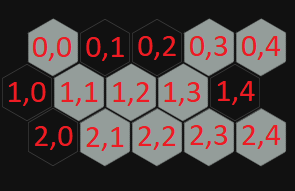
\includegraphics{hex_row_num.png}}
    \subfigure[Esempio coordinate con orientazione \textbf{col}]{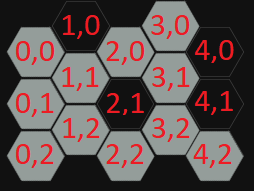
\includegraphics{hex_col_num.png}}
\end{center}    
\end{figure}

\paragraph{Geometria adiacente}
È utilizzata per poter rappresentare qualsiasi tipo di tabella creando un grafo bidirezionale, dove
i nodi sono le tessere e le connessioni sono degli oggetti connessione. \\ 
Non é possibile utilizzare il tag \lstinline|grid| per definire una geometria adiacente ma é 
necessario utilizzare il tag \lstinline|default| accoppiato
alla manipolazione manuale sia delle tessere che delle adiacenze di un gruppo.

\subsubsection{Tessera bianca}
La geometrie quadrate ed esagonali possiedono la tessera bianca che rappresenta lo spazio vuoto, 
definita tramite la lettera \lstinline|b| all'interno di un gruppo oppure tramite la tile \lstinline{BlankTile},
se si utilizza al di fuori della definizione di un gruppo.  

\subsubsection{Recuperare delle specifiche tessere}
Per accedere a una specifica tessera nei casi di geometrie regolari, si puó utilizzare la doppia
indicizzazione del gruppo, trattandolo come se fosse una matrice di tessere. \\
I significati dei due indici cambiano in base alla geometria del gruppo:
\begin{itemize}
    \item Quadrata: il primo indice è la colonna, il secondo è la riga
    \item Esagonale colonna: il primo indice è la colonna, il secondo é la riga
    \item Esagonale riga: il primo indice è la riga, il secondo è la colonna
\end{itemize}
Non è possibile accedere alle tessere di una geometria adiacente tramite indice poichè per definizione
non possiede una struttura regolare facilmente mappabile uno a uno con una griglia. 

\subsubsection{Default}
Il tag \lstinline|default <blocco istruzioni>| viene eseguito appena dopo l'istanziazione 
del gruppo in cui è definito. \\
Permette la modifica non standard di un gruppo, conferendo maggior controllo sulle relazioni tra le tessere 
e i gruppi.

\subsubsection{Connessioni tra tessere}
La connesione tra due tessere viene modellata tramite la classe specializzata:
\begin{lstlisting}
connection <Identificatori> <blocco attributo o funzione>
\end{lstlisting}
Possiede un attributo predefinito \lstinline|tile to| che deve essere popolato con la tessera 
destinataria della connessione.

\section{Ereditarietà}
Ereditarietà consente di definire delle classi derivate che ereditano o eseguono un override degli attributi, funzioni e azioni 
da una certa classe base
\paragraph{Ereditare da una classe base} 
Significa avere accesso a tutte le funzionalità della classe padre come se appartenessero alla classe figlia,
ovvero tramite l'operatore di auto riferimento \lstinline|this|.
\begin{lstlisting}
class base {}
class derived : base {}
\end{lstlisting}
\paragraph{Controllo sul tipo}
Un tipo derivato é anche dello stesso tipo di tutti i suoi tipi base, ovvero tutte le istanze
della classe figlia restituiranno il valore \lstinline|true| se confrontate con una classe 
antenata nella espressione di controllo del tipo. 

\subsection{Conversione del tipo}
Un tipo derivato é convertibile a un tipo antenato senza dover utilizzare l'operatore di casting,
questa operazione è chiamata "upcasting". \\
È importante sapere che le funzioni e le azioni chiamate dal tipo convertito avranno 
lo stesso comportamento che avrebbero se fossero chiamate su il tipo derivato. \\
Il caso contrario, il "downcasting" o conversione da tipo base a tipo derivato, è ammessa solamente
se in origine l'istanza era del tipo derivato o figlia del tipo derivato. 

\paragraph{Collezioni}
Le collezioni possono essere convertite ad altre collezioni il cui tipo che contengono segua 
comunque le regole di upcasting e downcasting sopra definite. 

\subsection{Override}
Override permette di ridefinire il comportamento di una funzione o azione modificandone
il tag effetto. \\ 
Per definire un override di una funzione é sufficiente definire nella classe derivante
un azione o funzione con lo stesso identificatore definito nella classe padre con la 
parola chiave \lstinline|override|:
\begin{lstlisting}
class Base 
{
    function A { 
        effect { // esegui istruzioni } 
    }
}

class Derived : Base
{
    override function A { 
        effect { // esegui altre istruzioni }
    }
}
\end{lstlisting}
Nell'effetto dell'override è possibile accedere agli stessi input dell'originale. 
Inoltre all'interno del blocco della classe derivata è possibile avviare la implementazione 
della base tramite il riferimento alla base \lstinline|base|, che racchiude
tutte le funzionalità definite nella classe padre. 

\section{Moltiplici file} \label{MultipleFiles}
L'utilizzo di piú di un file é supportato attraverso l'utilizzo di speciali sintassi
chiamate direttive d'importazione. 
\begin{lstlisting}
import "<percorso relativo al file>" [as <identificatore>];
\end{lstlisting}
Nella dichiarazione dell'importazione è possible assegnare un identificatore al file, 
attraverso il quale si accederà alle definizioni contenute all'interno di esso. \\
Nel caso sia omesso, tutte le definizioni all'interno del file importato non devono avere
conflitti con gli identificatori del file in cui si importano. \\
Le direttive d'importazione sono definibili solamente all'esterno di qualsiasi blocco,
prima di qualsiasi definizione o tag. 

\section{Punto di entrata}
L'entry point è definito tramite il tag setup nello stesso file in cui 
si utilizza la direttiva di gioco.
Dentro il blocco del tag si possono definire qualsiasi istruzioni che verrano eseguite
prima di far partire il primo turno di gioco.
\begin{lstlisting}
setup 
{
    <istruzione>
    <istruzione>
    ...
}
\end{lstlisting}

\section{Gestione della memoria}
Il linguaggio possiede una gestione automatica della memoria tramite garbage collector.

\subsection{Garbage Collector}
Il garbage collector si occupa di liberare la memoria allocata degli oggetti
che non possiedono nessun riferimento visible, recuperando la memoria utilizzata
per poterla riallocare in un momento futuro. \\ 
Internamente viene utilizzato un contatore che mantiene il numero di riferimenti 
allo stesso oggetto, quando si crea una copia del riferimento il contatore aumenta
pari al numero di copie create e viceversa decrementa quando un riferimento 
esce dalla visibiltá corrente.

\section{Esempio di utilizzo: Tris}
\begin{mdframed}[
    backgroundcolor=light-gray, 
    roundcorner=10pt,leftmargin=1, 
    rightmargin=1,
    innerleftmargin=15, 
    innertopmargin=15,
    innerbottommargin=15, 
    outerlinewidth=1, 
    linecolor=light-gray]
\lstinputlisting[language=tgpl_small]{./games/tris.tgpl}
\end{mdframed}

\section{Suggerimenti per l'implementazione}
Il linguaggio è stato formulato come linguaggio tradotto. 
In questa sezione vengono discusse delle possibili implementazioni 
supponendo come linguaggio bersaglio C\#, principalmente i due passaggi di 
traduzione dal linguaggio TGPL a CSharp e l'utilizzo dell'assembly compilato dal
codice generato.

\subsection{Traduzione}
I vari elementi del linguaggio sono tradotti ognuno in una equivalente 
struttura in c sharp.

\begin{lstlisting}[language=tgpl_small, caption=Codice in TGPL]
class Test
{
    action TestAction
    {
        input player Classe classe { ... }
        trigger OnChange { }
        effect { classe.Call(); }
    }

    function TestFunction
    {
        function input number N;
        return number;
        effect { return N * 2; }
    }
}
\end{lstlisting}
 
\begin{lstlisting}[style=sharpc_small, caption=Traduzione in CSharp]
// dichiarata in un file apposito
public class OnChange : EventBase { } 

public class Test
{
    public double test {get; set; } = 0;

    [EventTrigger(typeof(OnChange), 0)] // Type, priority
    [InjectedInput(typeof(Classe), "classe", ActionInputType.Player]
    public TGPLAction TestAction { get; }

    [FunctionInput(typeof(double), "N"]
    public TGPLFunction TestFunction()
    public double TestFunction(FunctionInput input) { get; }
}
\end{lstlisting}

\subsubsection{Eventi}
Gli eventi sono convertiti in una classe derivante da una classe base vuota utilizzata chiamata \lstinline|EventBase|,
la classe tradotta contiene tutti gli attributi sotto forma di proprietà publiche.

\subsubsection{Funzioni}
Le funzioni sono tradotte in una classe composta da due componenti, rispettivamente tradotti dal codice sorgente TGPL
\begin{lstlisting}[style=sharpc_small]
public class TGPLFunction
{
    public Dictionary<string, Func<ActionInput, bool>> Inputs {get; set;}
    public Action<InjectedInput> Effect {get; set;}
}
\end{lstlisting}
Per aiutare l'esecuzione del codice ogni proprietà di tipo \textit{TGPLFunction} è decorata  con degli attributi specifici 
rappresentanti i metadati della funzione, come i vari input da popolare. \\
\textit{Effect} é definito con argomento \textit{InjectedInput}, 
una classe contenente una collezione chiave-valore dove la chiave è l'identificatore dell'input
e il valore è l'oggetto inserito, popolato dall'\textit{InputInjector}. \\
Questo meccanismo è condiviso nella traduzione di qualsiasi input, cambiando solo la modalità
di acquisizione di esso dipendende dal modificatore definito.

\paragraph{Funzioni globali}
Le funzioni globali sono aggregate all'interno di una classe statica globale 
per fornire un accesso semplice al codice convertito.

\subsubsection{Azioni}
Le azioni sono tradotte in una classe composta da quattro componenti principali, rispettivamente tradotti dal codice sorgente TGPL:
\begin{lstlisting}[style=sharpc_small]
// attributi di input e di triggers in ordine di definizione
public class TGPLAction
{
    public List<Func<bool>> Requires {get; set;} 
    public List<Func<EventBase, bool>> Triggers {get; set;}
    public Dictionary<string, Func<ActionInput, bool>> Inputs {get; set;}
    public Action<InjectedInput> Effect {get; set;}
}
\end{lstlisting}
Per aiutare l'esecuzione del codice, come descritto in precedenza per \textit{TGPLFunction},
ogni proprietà di tipo Action è decorata con degli attributi specifici 
rappresentanti i metadati dell'azione, come gli eventi di trigger e i vari input da popolare.
vertite secondo le modalità descritte
precedentemente.

\paragraph*{Modificatori delle classi} I modificatori delle classi influenzano la traduzione:
\begin{itemize}
    \item \lstinline|local| viene tradotto con una proprietà Player associata rappresentante l'associazione al giocatore
    \item \lstinline|group| viene tradotto con una proprietà lista di player per rappresentare il gruppo di giocatori associato
    \item \lstinline|global| viene tradotta tramite la design pattern singleton, nello specifico possiede una proprietà statica che è l'istanza della classe
\end{itemize}

\subsubsection{Classi}
Le classi sono tradotte nell'equivalente in CSharp, dove gli attributi diventano 
proprietà publiche e le azioni e funzioni sono con
\subsection{Utilizzo della assembly generato}
Il secondo componente principale del software di traduzione si occupa di avviare 
il codice tradotto, ovvero di estrarre tutte le classi utili per l'esecuzione 
del gioco, detto anche \textit{ExecutionUnit} si compone di quattro componenti principali:
\begin{itemize}
    \item \textit{CodeProcessor}
    \item \textit{EventManager}
    \item \textit{InputInjector}
\end{itemize}

\subsubsection{InputInjector}
L'\textit{InputInjector} è il componente del processore con lo scopo di gestire la popolazione, secondo le specifiche del modificatore,
degli input utilizzati nelle varie azioni e funzioni. \\ 
Il comportamento di recupero di uno specifico input è definito dal relativo attributo di metadati \textit{InjectedInputAttribute},
in cui si definisce il tipo di oggetto, l'identificatore da utilizzare e la modalitá di recupero:
\begin{itemize}
    \item Player: dopo aver effettuato i filtri definiti richiede a un giocatore di scegliere l'input tramite l'interfaccia utente
    \item Auto: dopo aver effettuato i filtri popola direttamente l'input se valido
    \item Function: il valore é fornito direttamente dalla chiamata  
\end{itemize}

\paragraph{ReferenceRegistrar}
Il \textit{ReferenceRegistrar} ha il compito di mantenere tutti i riferimenti e il loro numero
creati durante l'esecuzione del gioco, è possibile concepirlo come dizionario CSharp:
\begin{lstlisting}[style=sharpc_small]
Dictionary<Type, List<(object, int)>>    
\end{lstlisting}
ovvero una collezione che associa a un certo tipo la lista degli oggetti creati durante l'esecuzione 
e il numero di riferimenti visibili. \\
Il registrar é principalmente interrogato dal \textit{InputInjector} durante la fase di recupero degli input
di una azione o funzione, restituendo in risposta alla richiesta del processore di tutte le istanze di un certo tipo 
per poterle filtrare secondo le specifiche dei filtri applicati a quell'input.

\subsubsection{EventManager}
L' \textit{EventManager} si occupa di mantenere, per ogni tipo di evento definito nel gioco, 
le azioni che ne sono in ascolto e il trigger specifico dell'azione associato all'evento ascoltato. 
Una delle possibili implementazioni è un semplice dizionario
\begin{lstlisting}[style=sharpc_small]
Dictionary<Type, List<(Action, Func<EventBase, bool>)>>
\end{lstlisting}
interrogato dal processore per recuperare le azioni correlate a uno specifico evento generato all'interno di un blocco d'istruzioni.
L'\textit{EventManager} risponde alla richiesta del processore con la lista delle azioni e del trigger associato. \\ 
In questa semplice implementazione, a ogni istanziazione di una classe contenente azioni è necessario registrare nell'EventManager
i triggers dell'azione. Ovviamente non è un sistema ottimizzato: un modo piú efficiente sarebbe creare dei metadati di ogni azione definita 
all'interno della classe, che ne descriva i filtri utilizzati nel flusso di esecuzione delle azioni.
I metadati conterrebbero non solo le informazioni per i triggers ma anche per i require e gli input dell'azione associata.
Nondimeno, a scopo di mantenere semplice la implementazione suggerita e, di conseguenza, la sua descrizione, 
si é scelto di optare per la versione meno efficiente.

\subsubsection{CodeProcessor}
L'\textit{CodeProcessor} é il responsabile di eseguire effettivamente le istruzioni contenute nei blocchi tradotti, durante l'esecuzione 
di un blocco se si presenta una generazione di eventi (sincrona o asincrona) la gestisce con le tecniche opportune:
\begin{itemize}
    \item Sincrona: blocco dell'esecuzione fino a risoluzione dell'intero albero degli eventi
    \item Asincrona: posticipazione dell'esecuzione dell'albero degli eventi alla termine del blocco corrente
\end{itemize}
In entrambi le modalità contatta l'\textit{EventManager} che gli restituisce la lista di tutte le azioni in ascolto di un certo evento,
per ogni azione contenuta all'interno della risposta del gestore degli eventi si avvia il flusso azione:

\paragraph{Flusso azione} Il flusso azione si divide in x passaggi principali:
\begin{enumerate}
    \item Valutazione dei require, ovvero se l'azione è attivata oppure disattivata
    \item Nel caso sia attivati si procede con la valutazione del trigger associato all'evento
    \item Se positiva si recuperano gli input tramite l'\textit{InputInjector}
    \item Se non si sono presentate eccezioni si esegue effetto dell'azione
    \item Infine se al suo interno sono presenti degli eventi generati si risolvono
\end{enumerate}

\paragraph{Interfaccia utente} Il processore utilizza un interfaccia utente dell'applicativo per mostrare informazioni
di esecuzione o gioco necessarie al giocatore, come il tabellone.